\section{Описание практической части}
\label{sec:Chapter4} \index{Chapter4}

Так как тема данной работы связана с активным использованием техник глубокого обучения, реализация всех методов и экспериментов
сделана на языке программирования \textit{Python}, который предоставляет все необходимые библиотеки, а именно:
\begin{itemize}
    \item \textit{Pillow}, \textit{opencv-python} -- для работы с изображениями, в т.ч. отрисовки шрифтов на изображении;
    \item \textit{albumentations}, \textit{augmixations} -- содержат реализацию основных методов аугментации изображений;
    \item \textit{pandas} -- для удобной работы с табличными данными, в частности для работы с информацией о размеченных наборах данных;
    \item \textit{scikit-learn}, \textit{scikit-image}, \textit{torch}, \textit{torchvision}, \textit{transformers} -- библиотеки с реализацией алгоритмов машинного обучения, а также основных метрик качества;
    \item \textit{datasets} -- для удобной загрузки наборов данных с \textit{huggingface.co}.
\end{itemize}

В рамках выполнения поставленной задачи было создано два публичных репозитория на платформе \textit{github.com}:
\begin{itemize}
    \item \textit{HandwritingGeneration}\footnote{\url{https://github.com/NastyBoget/HandwritingGeneration}}, содержащий код метода генерации синтетических изображений рукописного текста на основе шрифтов;
    \item \textit{hrtr}\footnote{\url{https://github.com/NastyBoget/hrtr)}}, содержащий код загрузки и обработки наборов данных, а также запуска необходимых экспериментов.
\end{itemize}

Помимо этого, для хранения и удобной загрузки созданных синтетических наборов данных использовалась платформа \textit{huggingface.co},
предоставляющая возможность бесплатно загружать и хранить файлы больших размеров.

В следующих секциях дано описание деталей реализации генерации изображений текста на основе рукописных шрифтов,
создания и публикации сгенерированных синтетических наборов данных, а также запуска экспериментов.


\subsection{Реализация генератора изображений рукописного текста}
\label{subsec:handwriting-generation}

В секции~\ref{subsec:synthetic} описан метод полу-автоматической генерации рукописных шрифтов, а также создания синтетических изображений на основе шрифтов.
Для этого был реализован набор модулей с классами-генераторами, доступный по ссылке \url{https://github.com/NastyBoget/HandwritingGeneration}.
На рисунке~\ref{fig:diagram_handwriting_generation} представлена диаграмма реализованных классов.

\begin{figure}[h!]
    \centering
    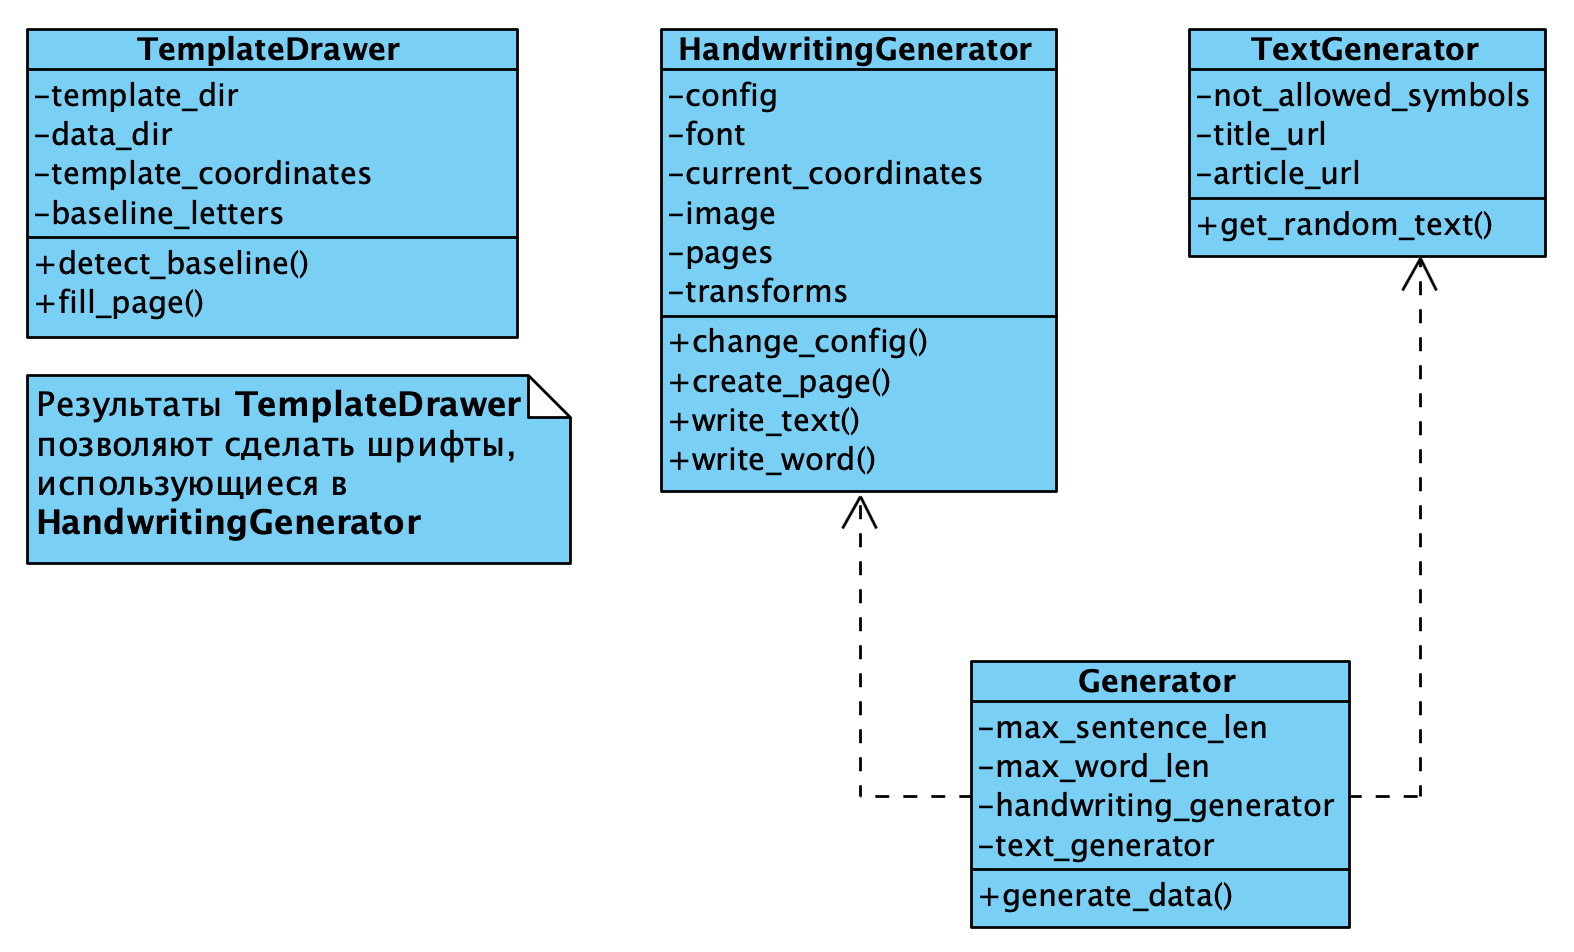
\includegraphics[width=\textwidth]{img/diagram_handwriting_generation}
    \caption{Диаграмма классов модуля генерации изображений рукописного текста}
    \label{fig:diagram_handwriting_generation}
\end{figure}

Показанные на рисунке~\ref{fig:diagram_handwriting_generation} классы позволяют осуществлять следующее:
\begin{itemize}
    \item \textit{TemplateDrawer} -- заполнение шаблона для приложения \textit{calligraphr}\footnote{\url{https://www.calligraphr.com}} для создания рукописных шрифтов;
    \item \textit{HandwritingGenerator} -- создание изображений рукописного текста с возможностью рандомизации стиля написания и фона;
    \item \textit{TextGenerator} -- генерация случайных текстов методом скачивания статей из Википедии\footnote{\url{https://ru.wikipedia.org}} и их очистки от неподдерживаемых символов;
    \item \textit{Generator} -- непосредственно генерация синтетического набора данных, включая генерацию текстов с их последующей отрисовкой.
\end{itemize}

Полученная реализация позволяет отрисовывать набор символов русского алфавита вместе с цифрами в среднем за 0.6 секунды
на компьютере MacBook Pro с процессором 1.4GHz Quad-Core Intel Core i5 и памятью 8GB 2133MHz LPDDR3.
Временная оценка работы генератора текста варьируется в зависимости от скорости работы сети, а также от длины статей, получаемых случайным образом.


\subsection{Реализация экспериментальной части}
\label{subsec:hrtr}

Реализация экспериментов, результаты которых описаны в секции~\ref{subsubsec:experiments_results}, находится в репозитории \url{https://github.com/NastyBoget/hrtr}.
В него включен отредактированный код моделей AttentionHTR и трансформера, а также их обучения и оценки качества распознавания.
Кроме того, важной частью является предварительная работа с данными -- их загрузка и приведение к унифицированному виду.
Для этого в репозитории есть специальный модуль, описанный в секции~\ref{subsubsec:datasets-processing}.
Далее более подробно описана реализация экспериментальной части.

\subsubsection{Создание и публикация дополнительных обучающих наборов данных}
\label{subsubsec:datasets-processing}

Прежде чем приступить к обучению моделей распознавания, необходимо иметь обучающий набор данных, представленный с специальном виде.
Для этого на языке \textit{Python} реализован модуль \textit{process\_datasets}, в котором каждый набор данных обрабатывается отдельным классом.
Диаграмма реализованных классов представлена на рисунке~\ref{fig:diagram_process_datasets}.

\begin{figure}[h!]
    \centering
    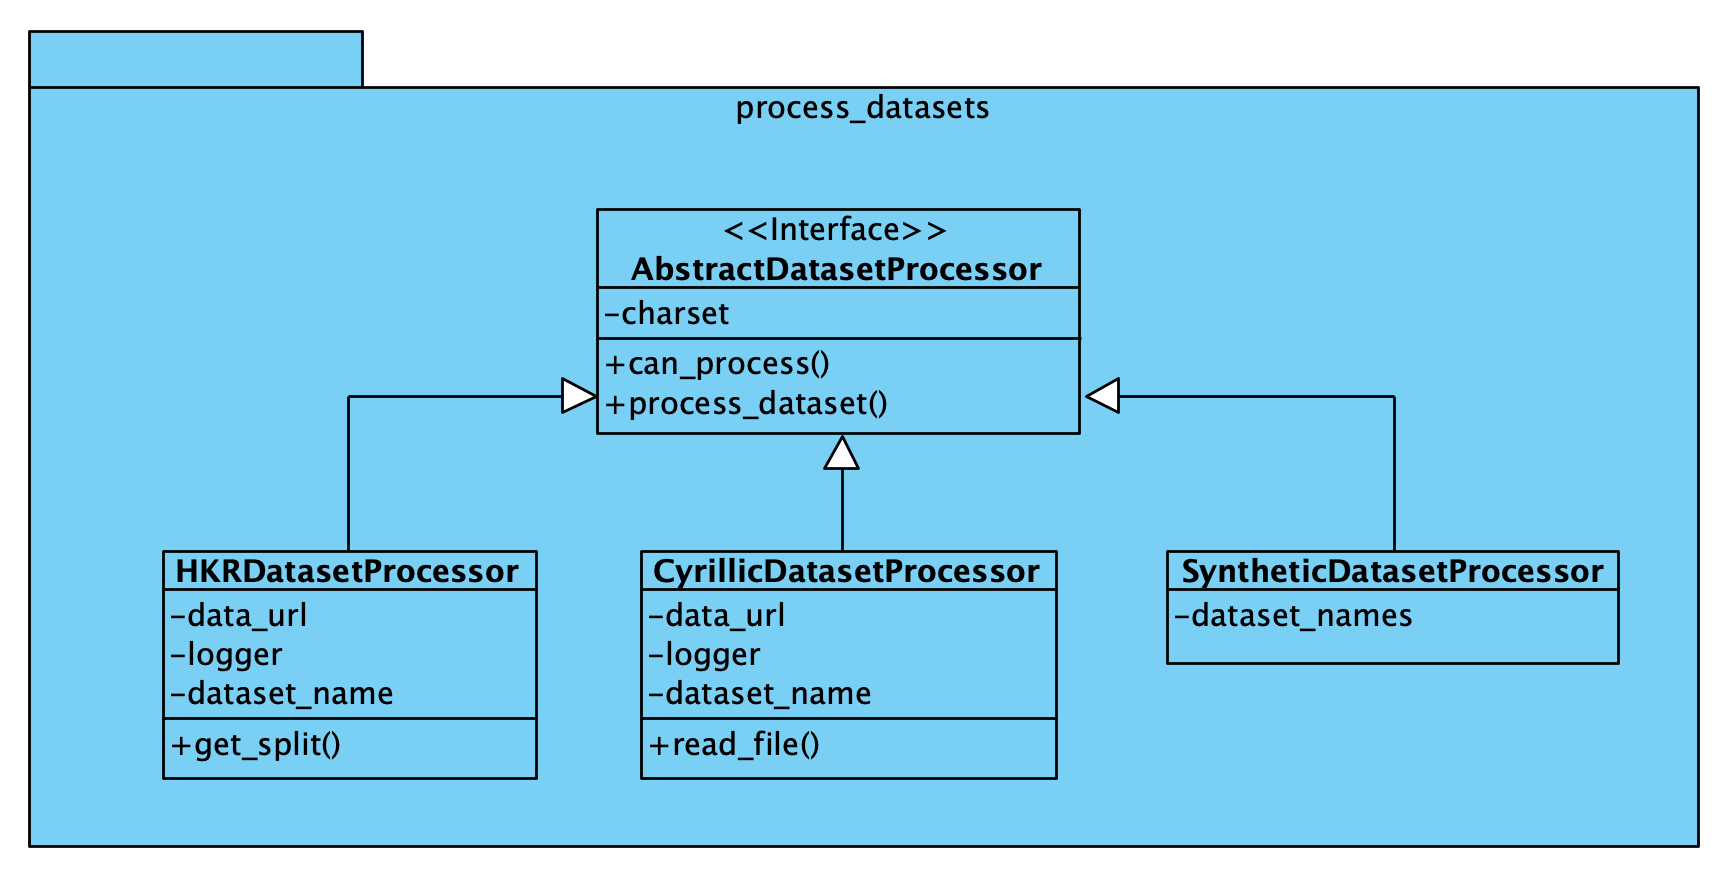
\includegraphics[width=\textwidth]{img/diagram_process_datasets}
    \caption{Диаграмма классов модуля загрузки и обработки наборов данных}
    \label{fig:diagram_process_datasets}
\end{figure}

Классы \textit{HKRDatasetProcessor} и \textit{CyrillicDatasetProcessor} используются для загрузки и обработки наборов данных HKR и Cyrillic Handwriting Dataset соответственно.
Класс \textit{SyntheticDatasetProcessor}, изображенный на рисунке~\ref{fig:diagram_process_datasets}, отвечает за обработку дополнительных наборов данных, сгенерированных автоматически.
В нём происходит загрузка наборов данных с \url{https://huggingface.co}, процесс генерации которых описан в главе~\ref{sec:Chapter3}, а именно:
\begin{itemize}
    \item Дополнение набора HKR сгенерированными данными с помощью шрифтов\footnote{\url{https://huggingface.co/datasets/nastyboget/synthetic_hkr}};
    \item Дополнение набора HKR сгенерированными данными с помощью Stackmix\footnote{\url{https://huggingface.co/datasets/nastyboget/stackmix_hkr}};
    \item Дополнение набора HKR сгенерированными данными с помощью ScrabbleGAN\footnote{\url{https://huggingface.co/datasets/nastyboget/gan_hkr}};
    \item Дополнение набора Cyrillic Handwriting Dataset сгенерированными данными с помощью шрифтов\footnote{\url{https://huggingface.co/datasets/nastyboget/synthetic_cyrillic}};
    \item Дополнение набора Cyrillic Handwriting Dataset сгенерированными данными с помощью Stackmix\footnote{\url{https://huggingface.co/datasets/nastyboget/stackmix_cyrillic}};
    \item Дополнение набора Cyrillic Handwriting Dataset сгенерированными данными с помощью ScrabbleGAN\footnote{\url{https://huggingface.co/datasets/nastyboget/gan_cyrillic}};
\end{itemize}

Для удобной загрузки и распаковки синтетических данных \textit{huggingface.co} предлагает API, которое позволяет с помощью
скрипта на языке \textit{Python} задать принцип, по которому формируется загружаемый набор данных.
На основе этого скрипта библиотека \textit{datasets} позволяет загружать и приводить данные к заданному виду при помощи одной строки кода.
Таким образом, для каждого из наборов был написан соответствующий скрипт, а класс \textit{SyntheticDatasetProcessor}
завершает более специфическую обработку данных в контексте других наборов.


\subsubsection{Обучение и оценка качества моделей распознавания}
\label{subsubsec:models-train-evaluation}

При наличии загруженных наборов данных можно приступать к обучению и оценке качества моделей распознавания рукописного текста.
Описание реализации архитектур двух моделей распознавания рукописного текста, их обучения и оценки качества представлено на рисунке~\ref{fig:diagram_hrtr}.

\begin{figure}[h!]
    \centering
    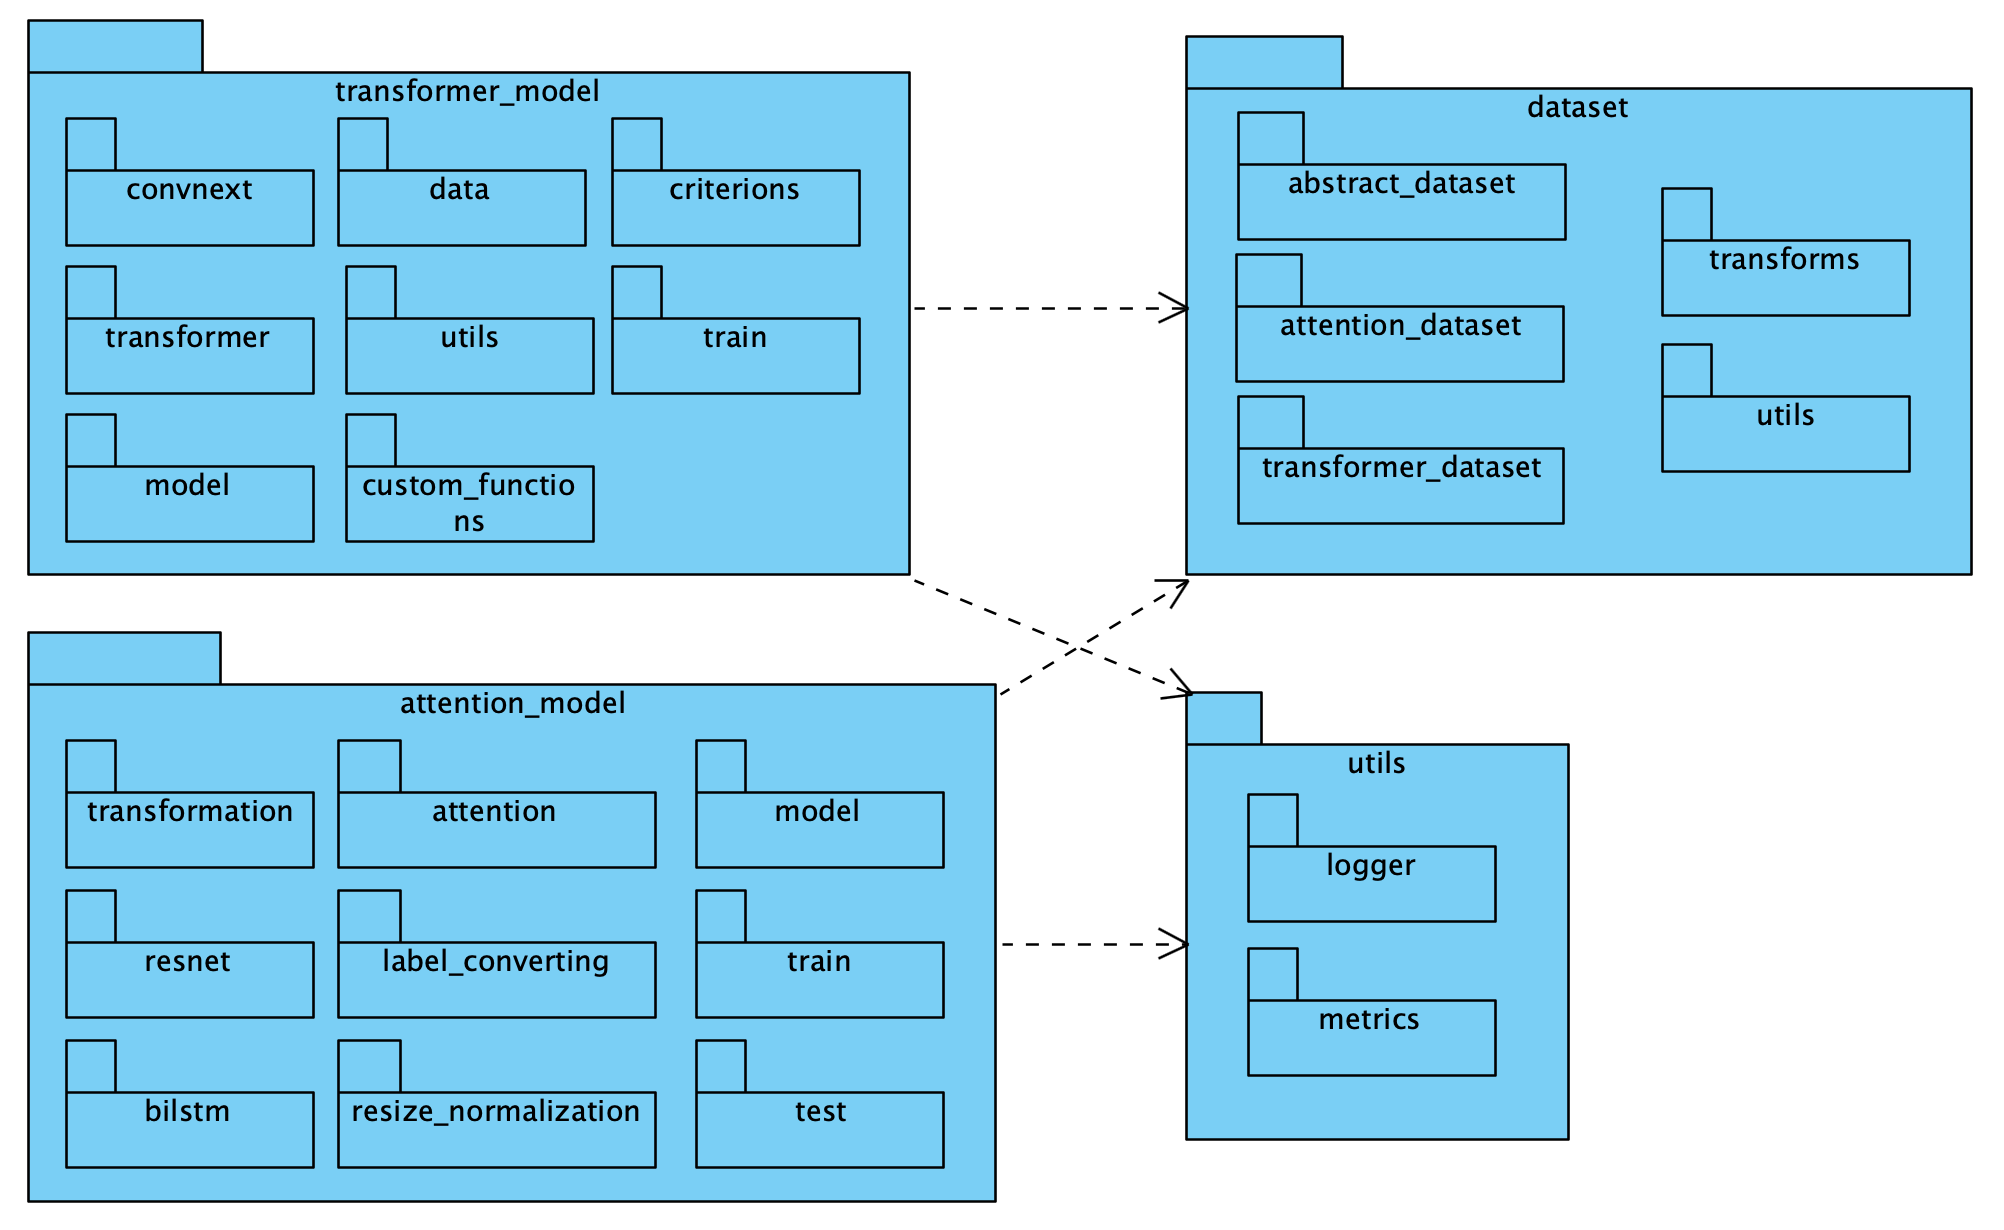
\includegraphics[width=\textwidth]{img/diagram_hrtr}
    \caption{Диаграмма пакетов для реализации обучения моделей и оценки качества}
    \label{fig:diagram_hrtr}
\end{figure}

Рисунок~\ref{fig:diagram_hrtr} описывает следующую структуру исходного кода:
\begin{itemize}
    \item Пакет \textit{utils} содержит вспомогательный код для логгирования процесса создания наборов данных и обучения,
    а также реализацию метрик оценки качества.
    Данный код написан самостоятельно для облегчения проведения всех необходимых экспериментов.
    \item Пакет \textit{datasets} содержит переопределение класса \textit{Dataset} библиотеки \textit{torch},
    сделанное для осуществления равномерной выборки данных их разных наборов в процессе обучения.
    Данный пакет содержит адаптеры, позволяющие специфичным образом обрабатывать данные для выбранных моделей распознавания.
    Помимо этого, в пакете находится фиксированный набор аугментаций, использующийся при обучении моделей,
    а также вспомогательная функция определения символьного набора данных.
    Данный пакет также реализован самостоятельно.
    \item Пакет \textit{attention\_model} содержит модифицированный код модели AttentionHTR\footnote{\url{https://github.com/dmitrijsk/AttentionHTR}}
    распознавания текста на английском языке.
    Составляющие пакета описывают архитектуру модели: модуль трансформации, модуль извлечения признаков resnet,
    модуль разметки последовательности bilstm, а также модуль декодирования attention.
    Модуль model позволяет собрать все предыдущие воедино, label\_converter используется для преобразования символов в численное представление и обратно,
    resize\_normalization используется для предобработки изображений перед их подачей на вход сети.
    Модули train и test используются для обучения модели и оценки результатов ее обучения соответственно.
    \item Пакет \textit{transformer\_model} содержит модифицированный код модели трансформер\footnote{\url{https://github.com/t0efL/end2end-HKR-research}}
    распознавания текста на английском и русском языках.
    Составляющие пакета convnext, transformer и model содержат реализацию архитектуры модели, data позволяет кодировать и декодировать символьные метки для изображений,
    custom\_functions, criterions и utils используются в процессе обучения модели, который реализован в модуле train.
    Там же находится код для оценки качества обученной модели.
\end{itemize}

Таким образом, реализованы все необходимые инструменты, использующиеся для проведения экспериментов и получения численных результатов
для сравнения методов генерации дополнительных обучающих наборов данных.

\subsection{Выводы}
\label{subsec:prac_conclusions}

В результате проделанной работы был реализован генератор изображений рукописного текста для русского языка на основе шрифтов\footnote{\url{https://github.com/NastyBoget/HandwritingGeneration}}.
Этот способ наряду с существующими реализованными методами был использован для получения дополнительных обучающих данных,
сформированные синтетические наборы находятся в открытом доступе на сайте \url{https://huggingface.co}.
Для проведения экспериментов реализованы модули обработки и унификации наборов данных, а также скрипты обучения и
оценки качества моделей распознавания рукописного текста.
Исходный код всех экспериментов находится в публичном доступе\footnote{\url{https://github.com/NastyBoget/hrtr}},
что позволяет воспроизвести полученные в работе результаты.